\documentclass[aspectratio=169,10pt]{beamer}
\usetheme{Madrid}
\usecolortheme{default}
\setbeamertemplate{navigation symbols}{}
\setbeamertemplate{footline}[frame number]
\usepackage{xeCJK}
\setCJKmainfont[BoldFont={PingFang SC Semibold}]{PingFang SC}
\setCJKsansfont[BoldFont={PingFang SC Semibold}]{PingFang SC}
\xeCJKDeclareCharClass{CJK}{"2192,"2260,"2194,"21D2,"00D7}
\usepackage{fontspec}
\setsansfont{Helvetica Neue}
\usepackage{amsmath,amssymb,booktabs,mathtools,graphicx,hyperref}
\usepackage{tikz}
\usetikzlibrary{arrows.meta,positioning}
\definecolor{positive}{HTML}{0173B2}
\definecolor{negative}{HTML}{DE8F05}
\definecolor{emphasis}{HTML}{029E73}
\definecolor{neutral}{gray}{0.55}
\definecolor{navy}{HTML}{1F3A5F}
\setbeamercolor{structure}{fg=navy}
\setbeamercolor{palette primary}{bg=navy,fg=white}
\setbeamercolor{palette secondary}{bg=navy!80,fg=white}
\setbeamercolor{palette tertiary}{bg=navy!60,fg=white}
\newcommand{\pos}[1]{\textcolor{positive}{#1}}
\newcommand{\con}[1]{\textcolor{negative}{#1}}
\newcommand{\HL}[1]{\textcolor{emphasis}{#1}}
\newcommand{\en}[1]{{\footnotesize\textcolor{neutral}{#1}}}

\title[Agent × Robot]{Agent × Robot：从 Harness 到自进化物理智能体}
\subtitle{四份材料的解读 · 23 条主线的 2026 综述 · 十条洞见}
\author{awesome\_agentic\_robot · asimfish}
\institute{github.com/asimfish/awesome\_agentic\_robot}
\date{2026-09-06}

\begin{document}

\begin{frame}
\titlepage
\end{frame}

\begin{frame}{一个问题：Harness 之后是什么？}
过去一年的关键词：VLA、WAM；最近的关键词：Agent、Harness。
\begin{itemize}
  \item 四份材料给出同一判断：它们不是互相替代，而是在拼装同一台机器人系统
  \item 本报告核实 154 篇论文（42 核心 / 94 扩展 / 18 基础）后回答三个问题：
  \begin{itemize}
    \item 2026 年 Agent × Robot 到底发生了什么
    \item 每份材料说对了什么、漏了什么
    \item 哪些判断有论文证据，哪些还是预测
  \end{itemize}
\end{itemize}
\begin{block}{结论先行}
下一阶段不是 Model Scaling，也不只是 Harness Scaling，而是 \HL{System Scaling + Experience Scaling}：先训练出足够好的机器人让它开始工作，再让工作本身继续训练机器人。
\end{block}
\en{Source materials: the Xiaohongshu essay by 具身RL日记, the Code-as-Policy deck, the 23-line retrieval map, and Lilian Weng's Lil'Log posts (2023, 2026).}
\end{frame}

\begin{frame}{五个结论}
\begin{columns}[T]
\column{0.48\textwidth}
\begin{enumerate}
  \item \textbf{优化对象在上移}：策略代码 → skill.md / 策略仓库 / 训练配方 / harness
  \item \textbf{冻结 VLA + 外围学习成为默认}：Harness VLA、BATON、AGM、HyMeS、Zetta；天花板由 LWD、Q-Planning 划出
  \item \textbf{验证器是新瓶颈也是新 scaling 轴}
\end{enumerate}
\column{0.48\textwidth}
\begin{enumerate}
  \setcounter{enumi}{3}
  \item \textbf{Harness 变成实时系统问题}：控制 / 计算 / 通信三处介入；Cloud can think, edge must survive
  \item \textbf{群体是经验规模化的出路，收益亚线性}：8 倍机器人 → 2--3 倍加速（ENPIRE）
\end{enumerate}
\vspace{4pt}
\[ z_{t+1} = A(z_t,\ \tau_t,\ r_t,\ \log_t) \]
\en{$z$: skill.md, policy.py, skill library, recipe, harness code; $A$: coding agent; $\tau$: rollouts; $r$: verification; $\log$: diagnosable evidence.}
\end{columns}
\end{frame}

\begin{frame}{解读一：小红书长文的 L1--L7 自进化分层}
\begin{center}
\vspace{4pt}
\small
\begin{tabular}{@{}lll@{}}
\toprule
层级 & 代表工作 & 被更新的对象 \\
\midrule
L1--L2 Retry / Replan & AgenticLab · Agentic Robot · MALMM · REMAC & 当前计划 \\
L3 Reflection & PhysReflect-VLA · Agentic RAG-VLM（14 类失败） & 纠正指令 \\
L4 Memory Evolution & Harness VLA“使用说明书” · AGM · OnEvoMemory & 记忆与适用范围 \\
L5 Skill Evolution & ASPIRE · ViReSkill · PRACTICE · SkillGLoW · RATs & 技能库 \\
L6 Policy Evolution & LWD · Q-Planning · Z-1 · TEMPO · Temporal GRPO & 策略权重 \\
L7 Fleet Evolution & LWD 16 台 · ENPIRE 8 工位 · RoboOS-NeXT & 群体共享数据 \\
\bottomrule
\end{tabular}
\end{center}
\begin{itemize}
  \item Retry ≠ Learning：真正的闭环是 Execution → Verification → Attribution → Reflection → Replan → Validation → Memory/Skill Update
  \item 2026 年正从 L2/L3 快速延伸到 L4--L7；\con{长文的盲区是治理与安全}
\end{itemize}
\end{frame}

\begin{frame}{解读一：六个“下一站”的证据核对}
\begin{center}
\vspace{4pt}
\small
\begin{tabular}{@{}p{2.5cm}p{8.1cm}l@{}}
\toprule
下一站 & 论文报告的数字 & 状态 \\
\midrule
Memory & RoboMME 16 任务 / 4 类记忆；PonderPounce 9B 60.83\% vs π0.5 17.93\% & \HL{实证} \\
Reflection \& Evolution & Harness VLA LIBERO-Pro +38.6pp（不改权重）；ASPIRE 零样本 31\% vs 4\% & \HL{实证} \\
双时间尺度 & Fast-in-Slow 117.7 Hz；StreamVLA 延迟 $-$48\%；CloudEdgeVLA 40 步延迟仍 63.8--78\% & \HL{实证} \\
Agent+VLA+RL & LWD 16 台机器人 95\%；Q-Planning 真机 40→90\%；RoboClaw 人工时间 $-$53.7\% & \HL{强证据} \\
Real→Sim→Learn→Real & TwinRL 20 分钟真机接近 100\%；PerceptTwin 计划成功率 +39\% & \HL{实证} \\
Multi-Robot 共享 & 两端有证据（RoboOS-NeXT 记忆、LWD 策略），中间层缺系统工作 & \con{部分预测} \\
\bottomrule
\end{tabular}
\end{center}
\en{Four of six claims are backed by 2026 papers; the fleet middle layers remain a prediction.}
\end{frame}

\begin{frame}{解读二：讲稿的五篇论文各在进化什么}
\begin{center}
\vspace{4pt}
\footnotesize
\begin{tabular}{@{}llll@{}}
\toprule
论文 & 外部状态 $z$ & 反馈 → 验证/选择 & 定位 \\
\midrule
Code as Policies '22 & policy code & 指令 + few-shot → 可执行 / 任务完成 & 提出范式 \\
SkillOpt '26.05 & skill.md & 打分 rollout → held-out 严格提升 & 自进化算法抽象 \\
CaP-X '26.03 & agent / benchmark & 执行反馈 / 视觉差分 → CaP-Bench & 研究平台 \\
ASPIRE '26.06 & 程序 + 技能库 & 多模态轨迹 → 验证过的修复 & 经验复用 \\
ENPIRE '26.06 & 训练代码 / 配方 / 基础设施 & 真机 rollout + 日志 → 物理成功 & 真机自动算法工程 \\
\bottomrule
\end{tabular}
\end{center}
\begin{itemize}
  \item Heuristic Learning：coding agent 依据反馈直接修改软件结构（策略、检测器、测试、配置、记忆）
  \item Lil'Log 的阶梯 prompt → context → workflow → harness code → optimizer code 在机器人侧被完整走了一遍
  \item 7--9 月续作：PRACTICE、SkillGLoW（技能库）；Zetta、SHAPER（运行时）；RHO（Repositories-as-Policies，部署时单轮执行）
\end{itemize}
\end{frame}

\begin{frame}{解读二：SkillOpt 把技能训练做成文本空间的梯度下降}
\begin{columns}[T]
\column{0.46\textwidth}
\begin{center}
\small
\begin{tabular}{@{}ll@{}}
\toprule
权重空间 & 文本空间 \\
\midrule
参数 & skill 文档 \\
梯度方向 & 轨迹抽出的编辑方向 \\
学习率 & 编辑预算 $L_t$ \\
验证 & held-out 选择门 \\
负样本 & 拒绝编辑缓冲区 \\
epoch & 慢速 / 元更新 \\
\bottomrule
\end{tabular}
\end{center}
\column{0.50\textwidth}
\textbf{52 / 52} cells 最优或并列（6 基准 × 7 模型 × 3 harness）
\begin{itemize}
  \item GPT-5.5：直接对话 +23.5、Codex +24.8、Claude Code +19.1
  \item 消融：去预算 77.5→75.7；去拒绝缓冲 →72.9；\con{去 epoch 元更新 →55.0}
  \item OfficeQA +39pp 来自单个被接受的编辑
  \item SkillOpt-Lite：零阶优化视角，推广到 HarnessOpt
\end{itemize}
\end{columns}
\end{frame}

\begin{frame}{解读二：ENPIRE 的四个真机教训}
\begin{columns}[T]
\column{0.48\textwidth}
\begin{block}{1 · 仿真成功 ≠ 真机鲁棒}
Gym-PushT：Codex/Claude 约 2 h 达 95\%；真实 Push-T：Codex ≈95\%，Claude ≈75\%，Kimi ≈60\%。摩擦漂移、位姿误差、控制器偏差。
\end{block}
\textbf{2 · 纯 BC 不够}：pin insertion 要求 50 次连续成功；hillclimb 最大一步是 BC regularization +10.8pp。
\column{0.48\textwidth}
\begin{block}{3 · 群体提升的是假设吞吐量}
1/4/8 台机器人：Push-T 收敛 5 h → 2 h；pin insertion 1.5 h+ → 40 min。8 倍机器人只有 2--3 倍加速。
\end{block}
\textbf{4 · 持续学习发生在文本记忆里}：研究总结写成 Markdown 传给新 Agent，刻意删除轨迹、checkpoint、日志。
\end{columns}
\vspace{6pt}
第五组：RoboCasa365 上 GR00T ≈53\%，\HL{ENPIRE 混合方案 ≈77\%}（代码做 hover pose，VLA 做接触），CaP-X ≈27\%。
\end{frame}

\begin{frame}{解读四：Lil'Log 的 Harness 理论 → 机器人侧对应物}
\begin{center}
\vspace{4pt}
\small
\begin{tabular}{@{}p{5.0cm}p{7.9cm}@{}}
\toprule
Lil'Log《Harness Engineering for Self-Improvement》 & 机器人侧 \\
\midrule
工作流自动化 plan→execute→observe→improve & ENPIRE reset→execute→verify→refine；ASPIRE；RoboClaw \\
文件系统即持久记忆 & PhyAgentOS State-as-a-File；ENPIRE Markdown 总结；AgenticRobotics \\
子代理与后台任务 & ENPIRE Agent 团队 × 集群；HARBOR；RATs \\
优化阶梯 prompt→…→optimizer code & SkillOpt · ASPIRE · RHO/SHAPER · Meta-Harness/HarnessOpt \\
Harness updating ≠ harness benefit & Codex/Claude/Kimi 的真机差距更像“利用 harness”的差距 \\
评估器与权限在演化循环之外 & Runtime Governance · ICAN-Deploy · 签名验证器 \\
\bottomrule
\end{tabular}
\end{center}
\en{Three essential differences of a robot harness (Thea; Harness Engineering for Physical AI): reading world state is hard, judging outcomes is hard, and time matters.}
\end{frame}

\begin{frame}{解读三：23 条主线的密度与状态}
\begin{columns}[T]
\column{0.32\textwidth}
\textbf{最密集（6--8 月）}
\begin{itemize}
  \item T15 Harness：RHO、Harness VLA、Thea、Guava、HARBOR、Zetta、SHAPER
  \item T5 Memory：RoboMME、PonderPounce、AGM、HyMeS、BATON、NativeMEM
  \item T9 VLA+RL：Temporal GRPO、TEMPO、WCM、Z-1、ARLI
\end{itemize}
\column{0.32\textwidth}
\textbf{快速成熟}
\begin{itemize}
  \item T13 双系统：UniFS、Latent Bridge、VisualThink-VLA
  \item T11 数字孪生：RoboSnap、Agentic Real2Sim、PerceptTwin
  \item T16/T17 治理与安全：Runtime Governance、EmbodiedGovBench、EMBGuard、VASO
\end{itemize}
\column{0.32\textwidth}
\textbf{仍在早期}
\begin{itemize}
  \item T21 Fleet：中间的共享经验 / 世界知识缺系统工作
  \item T18 标准接口：MHS（2026-08-27）与 ROS 2 Harness Profile 待融合
  \item T22 主动感知：PhysCaP、ActiveVLA，成本控制是关键
\end{itemize}
\end{columns}
\vspace{4pt}
\en{Full line-by-line survey in report Section 4; 154 papers by line in README.}
\end{frame}

\begin{frame}{解读三：长程任务被重述为“技能交接问题”}
\begin{columns}[T]
\column{0.48\textwidth}
\textbf{BATON 的两个诊断}
\begin{itemize}
  \item 整任务探索代价 $T^K$，失败无法归因 → 以子任务为探索单元，代价 $T\cdot K$
  \item VLA 原语只有退出条件、没有进入条件 → 转移感知记忆治理调用 / 交接 / 前瞻
  \item RoboMemArena 任务成功 +11.6\%，不更新参数
\end{itemize}
\en{AtomBridge: +10--25\% on 8-step sequences; Foresight Residual RL: 85.6\% vs 54.5\%.}
\column{0.48\textwidth}
\textbf{T23 验证器成为瓶颈}
\begin{itemize}
  \item PhyAgentOS SessionVerifier：执行终止 ≠ 语义完成
  \item Thea：Evaluation as Exit Codes
  \item AGM：2.43M 参数验证头，物理证据才推进进度
  \item LLM-as-a-Verifier：RoboRewardBench 87.4\%，可作 RL 密集奖励
  \item VASO：模型检查反例 → 技能契约的文本梯度
  \item 立场论文：成功率无法区分语义匹配与物理泛化
\end{itemize}
\end{columns}
\end{frame}

\begin{frame}{解读三：“可治理”从论文变成工程}
\begin{columns}[T]
\column{0.48\textwidth}
\begin{block}{Runtime Governance（Harnessing Embodied Agents）}
1000 次随机试验 \textbf{96.2\%} 越权拦截；运行时漂移下不安全继续 100\%→22.2\%；恢复成功 90.7\%；唯一提供持续运行时检测（RVDR 61.3\% vs 0\%）。
\end{block}
\textbf{EmbodiedGovBench 七维}：越权调用 · 运行时漂移 · 恢复 · 策略可移植 · 升级安全 · 人工接管 · 审计完整性
\column{0.48\textwidth}
\textbf{被忽略的层面}
\begin{itemize}
  \item Same Weights, Different Robot：换一个动作反归一化元数据键，LIBERO-Goal 28/28 → 2/28
  \item 多机器人通信攻击：最高 97.8\% 不安全动作成功率；CPV Gate 70.0\%→36.6\%
  \item MHS（Anthropic 2026-08-27）：agent 标准化接入真实设备，“硬件版 MCP”
\end{itemize}
\end{columns}
\end{frame}

\begin{frame}{综合：Goal → Action → Experience → Learning → Better Action}
\begin{center}
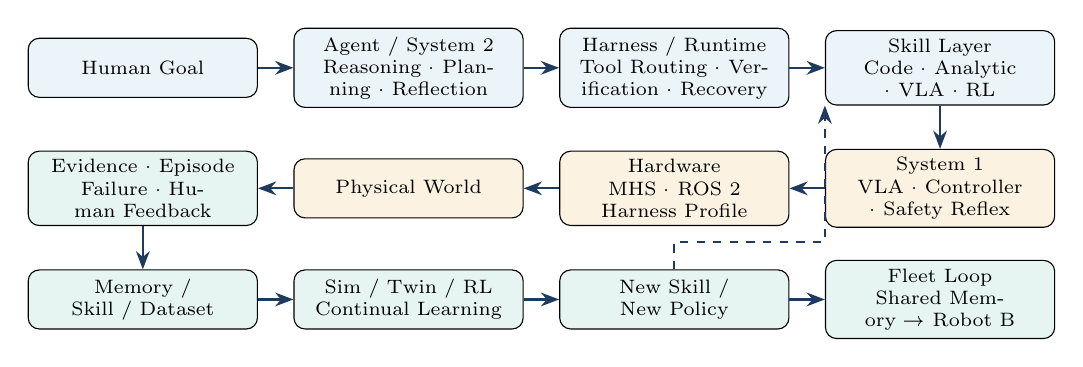
\begin{tikzpicture}[
  box/.style={draw, rounded corners, text width=2.7cm, minimum height=0.75cm, inner sep=3pt, font=\scriptsize, align=center, fill=positive!8},
  gbox/.style={box, fill=emphasis!10},
  obox/.style={box, fill=negative!12},
  arr/.style={-{Stealth}, thick, navy}
]
  \node[box] (goal) {Human Goal};
  \node[box, right=0.45cm of goal] (agent) {Agent / System 2\\Reasoning · Planning · Reflection};
  \node[box, right=0.45cm of agent] (harness) {Harness / Runtime\\Tool Routing · Verification · Recovery};
  \node[box, right=0.45cm of harness] (skill) {Skill Layer\\Code · Analytic · VLA · RL};
  \node[obox, below=0.55cm of skill] (fast) {System 1\\VLA · Controller · Safety Reflex};
  \node[obox, left=0.45cm of fast] (hw) {Hardware\\MHS · ROS 2 Harness Profile};
  \node[obox, left=0.45cm of hw] (world) {Physical World};
  \node[gbox, left=0.45cm of world] (evidence) {Evidence · Episode\\Failure · Human Feedback};
  \node[gbox, below=0.55cm of evidence] (memory) {Memory / Skill / Dataset};
  \node[gbox, right=0.45cm of memory] (sim) {Sim / Twin / RL\\Continual Learning};
  \node[gbox, right=0.45cm of sim] (newpol) {New Skill / New Policy};
  \node[gbox, right=0.45cm of newpol] (fleet) {Fleet Loop\\Shared Memory → Robot B};
  \draw[arr] (goal) -- (agent); \draw[arr] (agent) -- (harness); \draw[arr] (harness) -- (skill);
  \draw[arr] (skill) -- (fast); \draw[arr] (fast) -- (hw); \draw[arr] (hw) -- (world); \draw[arr] (world) -- (evidence);
  \draw[arr] (evidence) -- (memory); \draw[arr] (memory) -- (sim); \draw[arr] (sim) -- (newpol); \draw[arr] (newpol) -- (fleet);
  \draw[arr, dashed] (newpol.north) -- ++(0,0.35) -| (skill.south west);
\end{tikzpicture}
\end{center}
三个闭环：\pos{Execution Loop}（这次能不能做完）· \HL{Learning Loop}（下次能不能更好）· \con{Fleet Loop}（一台学到的能不能变成群体的）
\end{frame}

\begin{frame}{十条洞见（上）}
\begin{enumerate}
  \item \textbf{优化对象上移}：贡献取决于把哪个层级的产物变成可搜索、可验证、可复用的对象
  \item \textbf{冻结 VLA + 外围学习是默认，但有天花板}：外围学不到“视觉→接触→力→微动作”；HyMeS 的分工——技能在权重里，记忆在代码里
  \item \textbf{验证器是新瓶颈也是新 scaling 轴}：一个更好的验证器比一个更好的规划器更稀缺
  \item \textbf{记忆分权重内 / 权重外两路}：精确时序与计数用权重内（NativeMEM 32.4→84.0\%）；跨会话、抗干扰、可编辑用结构化外部记忆
  \item \textbf{Harness 变成实时系统问题}：control-time Roofline、20 Hz 约束、延迟破坏马尔可夫假设；“harness 像 OS”在机器人侧是字面意义
\end{enumerate}
\end{frame}

\begin{frame}{十条洞见（下）}
\begin{enumerate}
  \setcounter{enumi}{5}
  \item \textbf{真机试错成本决定 Sim 是 sandbox}：Real→Sim→Learn→Verify→Real 每一步都有工具，缺的是串起来的 harness
  \item \textbf{治理与安全成为一等公民}：观点文章低估、论文（多在仿真）高估
  \item \textbf{群体是出路，收益亚线性}：价值在假设与场景的多样性，“多样性塌缩”以多个 Agent 试同一想法出现
  \item \textbf{Coding agent 成为 roboticist}：autoresearch 进入物理世界，附带三个约束——读状态难、判结果难、有时间
  \item \textbf{风险与反例}：harness updating ≠ harness benefit；验证器必须在可编辑面之外；对话可能降低多机器人任务成功；共享经验会共享污染
\end{enumerate}
\end{frame}

\begin{frame}{八个开放问题}
\begin{columns}[T]
\column{0.48\textwidth}
\begin{enumerate}
  \item 可扩展的分层验证器（连续评分 + 物理证据头 + 形式检查）
  \item 给每个原语学显式进入条件与交接质量，$T^K \to T\cdot K$
  \item 权重内 / 权重外记忆的分工，用 RoboMME 分类评测
  \item Projection / Isolation / Transfer 做成 ROS 2 Harness Profile 并对接 MHS
\end{enumerate}
\column{0.48\textwidth}
\begin{enumerate}
  \setcounter{enumi}{4}
  \item 群体多样性：新颖性拒绝采样 / 过程族去重
  \item Real→Sim→Verify→Real 流水线化
  \item 治理指标进入 LWD / ENPIRE 规模的真机集群
  \item 度量 Experience Scaling：TPH × MTBI、MRU/MTU、假阳性晋升率
\end{enumerate}
\end{columns}
\begin{block}{method-story 起点}
选一个 $z$（如技能的进入条件 + 验证头），选 $r$ 的来源（物理证据 + 形式检查），画清 $A$ 的可编辑面并把验证器放在外面，在 LIBERO-Pro Long / RoboMemArena 上报告库规模 vs 零样本成功率曲线。
\end{block}
\end{frame}

\begin{frame}{三个带走的判断}
\begin{enumerate}
  \item \textbf{自进化 = 优化外部产物 $z$}，区别只在 $z$ 是什么、$r$ 从哪来、$A$ 被允许改什么
  \item \textbf{验证器决定自进化循环的上限}——奖励作弊、过度乐观、“仿真 100\% 真机 60\%”都发生在这里
  \item \textbf{System Scaling + Experience Scaling}：先训练出足够好的机器人让它开始工作，再让工作本身继续训练机器人
\end{enumerate}
\vspace{8pt}
\en{Train a robot good enough to start working; then let the work keep training the robot.}
\end{frame}

\begin{frame}[allowframebreaks]{参考文献（核心）}
\small
\begin{thebibliography}{9}
\bibitem{cap} Liang et al. Code as Policies: Language Model Programs for Embodied Control. arXiv:2209.07753, 2022.
\bibitem{skillopt} Yang, Gong et al. SkillOpt: Executive Strategy for Self-Evolving Agent Skills. arXiv:2605.23904, 2026.
\bibitem{capx} Fu et al. CaP-X: A Framework for Benchmarking and Improving Coding Agents for Robot Manipulation. arXiv:2603.22435, 2026.
\bibitem{aspire} Lu et al. ASPIRE: Agentic Skills Discovery for Robotics. arXiv:2607.00272, 2026.
\bibitem{enpire} Xiao et al. ENPIRE: Agentic Robot Policy Self-Improvement in the Real World. arXiv:2606.19980, 2026.
\bibitem{harnessvla} Zhang et al. Harness VLA: Steering Frozen VLAs into Reliable Manipulation Primitives via Memory-Guided Agents. arXiv:2607.08448, 2026.
\bibitem{lwd} Wang et al. Learning While Deploying: Fleet-Scale RL for Generalist Robot Policies. arXiv:2605.00416, 2026.
\bibitem{phyagentos} Liu et al. PhyAgentOS: A Self-Evolving Operating System for Embodied Agents. arXiv:2607.16636, 2026.
\bibitem{hepai} Lee, Chae, Park. Harness Engineering for Physical AI: Robot Middleware Is the Harness Layer. arXiv:2606.09416, 2026.
\bibitem{weng} Weng, L. Harness Engineering for Self-Improvement. Lil'Log, July 2026; LLM Powered Autonomous Agents. Lil'Log, June 2023.
\bibitem{xhs} 具身RL日记. Harness 之后，Agent+Robot 下一站是什么？ 小红书, 2026.
\end{thebibliography}
\end{frame}

\begin{frame}
\centering
{\Large 谢谢 · Thank you}\\[8pt]
github.com/asimfish/awesome\_agentic\_robot\\[4pt]
\en{README（154 篇论文 / 24 主线）· 中英文报告 PDF · HTML 幻灯片 · SuperTranslate 中文译本}
\end{frame}

\appendix
\begin{frame}{Backup Slides}
\end{frame}

\begin{frame}{Backup：记忆的两条路线}
\begin{center}
\small
\begin{tabular}{@{}p{2.6cm}p{4.8cm}p{5.0cm}@{}}
\toprule
& 权重内记忆 & 权重外记忆 \\
\midrule
代表工作 & NativeMEM · LaMem-VLA · Remember Smarter · VQ-Memory · SkillMemo · PonderPounce & AGM · HyMeS · BATON · 概念中心记忆 · OnEvoMemory · RoboHarness \\
数字 & NativeMEM 32.4→84.0\%；Remember Smarter 53.6→70.6\% & HyMeS 41.3→60.1\%；AGM 只在物理证据后推进 \\
适用 & 精确时序、计数、低延迟 & 跨会话、抗干扰、可解释、可编辑 \\
依据 & RoboMME：记忆表示高度任务依赖 & RoboMME-Interference：感知型记忆随干扰衰减，检索可恢复 \\
\bottomrule
\end{tabular}
\end{center}
\end{frame}

\begin{frame}{Backup：五篇核心论文的中文译本（SuperTranslate）}
\begin{itemize}
  \item 引擎需要 LLM API；本机无可用 key，走引擎的手工翻译通路：\texttt{export} 导出文本块 → 人工译文表 → \texttt{cache-only} 原位回填 → \texttt{inspect} QA
  \item Code as Policies：正文全译（16 页），inspect 仅报 3 条附录页未翻译（刻意保留）
  \item SkillOpt / CaP-X / ENPIRE / ASPIRE：首页（标题、摘要、引言开头）
  \item CaP-X 与 ENPIRE 原文含 MuPDF 不支持的 CID 字体，先经 Ghostscript 重蒸馏
  \item \texttt{scripts/translate\_papers.sh}：配置 \texttt{DEEPSEEK\_API\_KEY} 后一键补全
\end{itemize}
\end{frame}

\begin{frame}{Backup：ENPIRE 群体加速为何亚线性}
\begin{itemize}
  \item 1 / 4 / 8 个 Agent 对应 1 / 4 / 8 台机器人，共享 Gym 接口、reward、reset、baseline 代码库
  \item Push-T 归一化 1.0：约 5 h → 约 2 h；pin insertion：1.5 h+ → 约 40 min
  \item 原因：Agent 重复探索相似想法、等待训练或大模型输出、阅读其他分支、整理合并实验、分析日志
  \item 提升的是 hypothesis throughput，不是同一策略的 rollout batch；对应 Lil'Log 的“多样性塌缩”
  \item ENPIRE 提出 Mean Robot Utilization / Mean Token Utilization 度量多 Agent 物理自动研究效率
\end{itemize}
\end{frame}

\end{document}
